\FloatBarrier
\section{Structural Inference from the Focal Model}

Section 5 settled the predictive question: on the corrected causal foundation, the structural Bayesian model M6 matches the unconstrained ensemble M5 to within 0.4 percentage points of MdAPE. This section reports what that tie purchases. M5's output is a prediction; M6's output is a posterior distribution over the parameters of the population relationship $P(Y \mid X)$ that the pipeline targets, and those parameters carry physical and policy meaning unavailable from any point prediction. Four parameters carry the section's empirical claims, and they were declared as the parameters of interest before any robustness fits were run (Section 6.5): $\beta_A$, the floor-area elasticity; $\beta_T$, the data-year trend; $\sigma_\alpha$, the between-type heterogeneity; and $\sigma$, the residual scale. The remaining slopes $\beta_B$ and $\beta_Y$ are auxiliary controls. Because M6 regresses the outcome on the upstream features alone, its slopes estimate the reduced form of the world layer: the composite causal path from building characteristics through energy use into emissions. All results in this section are drawn from the same fitted posterior evaluated in the factorial experiment: the trace was saved at fit time (4 chains, 3,000 post-warmup draws each) and re-loaded for this analysis, so every number here is consistent with Table 5.1 by construction.

\subsection{Posterior Health and Calibration}

Inference is only as good as the sample that carries it, so the diagnostics come first. Across all parameters, $\hat{R}_{\max} = 1.0095$ and $\text{ESS}_{\min} = 526$, within the $\hat{R} < 1.01$ and bulk ESS $> 400$ thresholds (\cit{vehtarietal2021}{Vehtari et al., 2021}), with zero divergent transitions across 12,000 draws. The slowest-mixing parameters are the global hyperparameters $\bar{\alpha}$ and $\sigma$; the 55 property-type offsets mix far faster ($\text{ESS}_{\min} = 11{,}409$), which is the expected signature of the non-centred parameterisation. The type-level offsets $\delta_j$ are nearly decorrelated by construction, while the global scalars must integrate over all type-level uncertainty.

The predictive side is checked by Pareto-smoothed importance-sampling leave-one-out cross-validation (PSIS-LOO; \cit{vehtarietal2017}{Vehtari et al., 2017}). The ELPD of $-12{,}316$ (SE $317.4$) reproduces the experiment's reported value exactly, confirming the loaded trace is identical to the posterior evaluated in the factorial. The Pareto-$k$ diagnostic flags observations whose removal would substantially change the posterior and for which the LOO approximation is unreliable: 1 of 21,406 observations exceeds $k = 0.7$, and 7 exceed $k = 0.5$. The median $k$ of $-0.060$ indicates that the typical held-out observation is, if anything, more consistent with the model than the average one, the opposite of overfitting. Interval calibration was already quantified in Table 5.1: 92.8\% empirical coverage at the 89\% nominal level, slightly conservative. Figure 6.1 overlays 200 posterior predictive replications on the observed outcome distribution on both the log and original scales.

\begin{figure}[tbp]
\centering
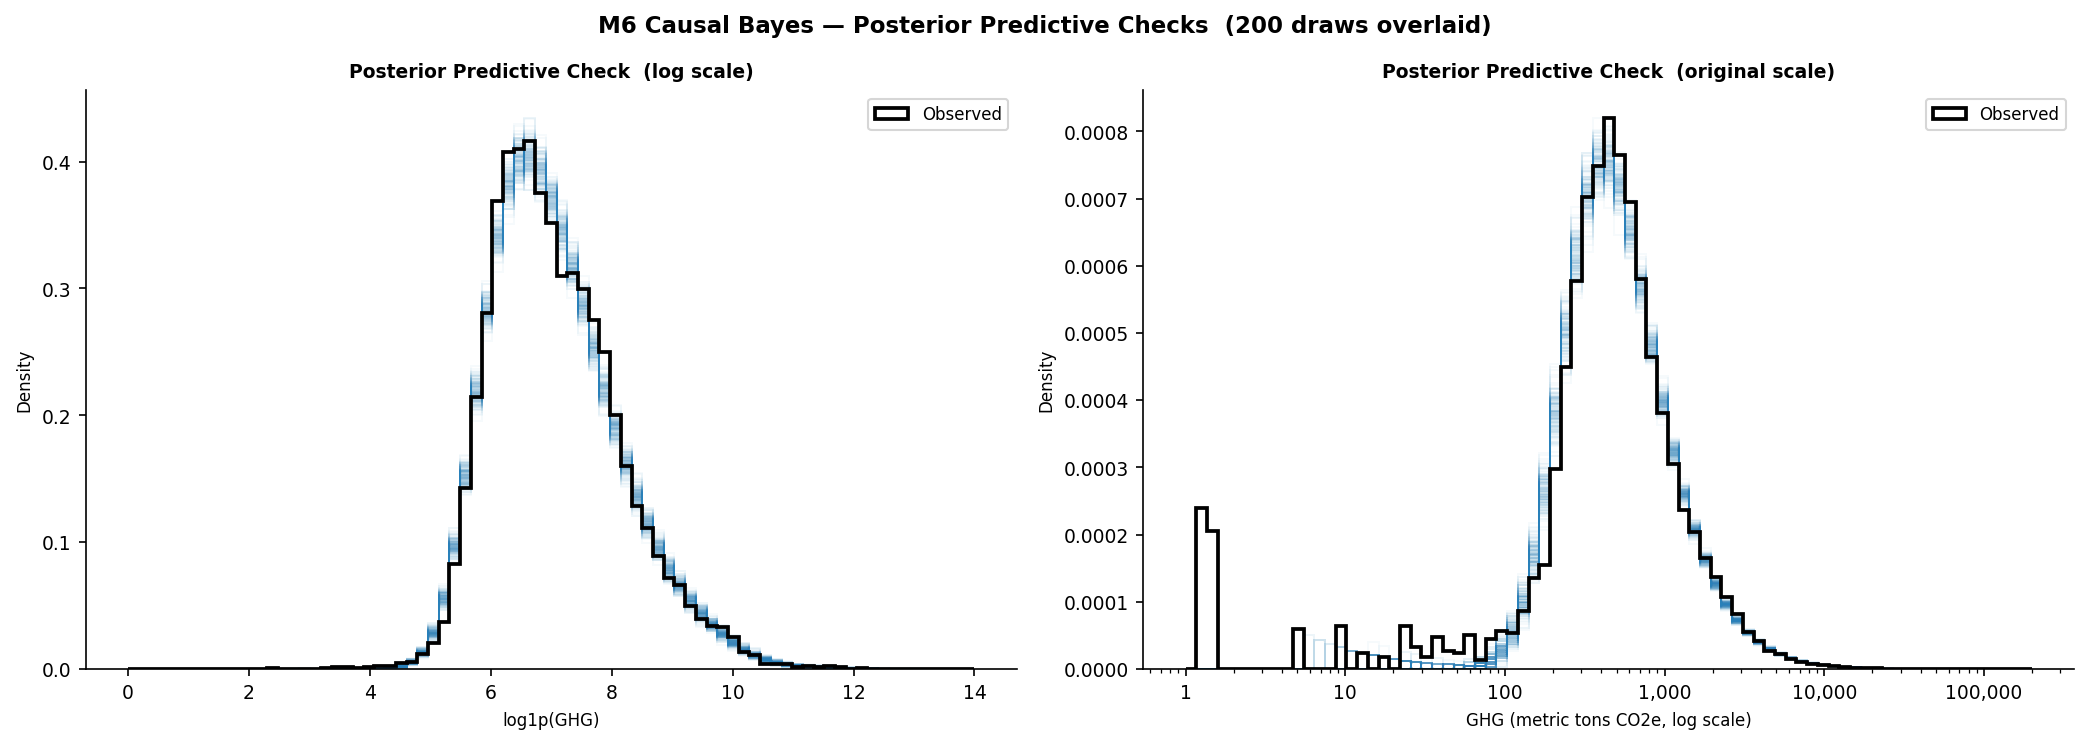
\includegraphics[width=0.95\linewidth]{figures/fig_ppc.png}
\caption*{\textbf{Figure 6.1. M6 posterior predictive check.} 200 datasets simulated from the posterior (blue) overlaid on the observed $\log_{1+}$(GHG) distribution (black), on the log scale (left) and the original scale with logarithmic axis (right). Author's analysis of Chicago Energy Benchmarking data.}
\end{figure}

\subsection{Global Parameter Posteriors}

Floor area and the temporal trend dominate the posterior, with substantial property-type heterogeneity and a precisely estimated residual scale. Table 6.1 reports all seven parameters with 89\% credible intervals; Figure 6.2 shows the forest plot.

\par\medskip\noindent
{\small\itshape \textbf{Table 6.1. M6 global parameter posteriors.} Posterior means and 89\% credible intervals for the seven scalar parameters of the generative model in Section 5.4. The four upstream slopes are the parameters of interest; $\bar{\alpha}$, $\sigma_\alpha$, and $\sigma$ are the hierarchy's location, spread, and residual scale. Author's analysis of Chicago Energy Benchmarking data.\par}
\nopagebreak\medskip\nopagebreak
{
\setlength{\tabcolsep}{7pt}
\renewcommand{\arraystretch}{1.15}
\begin{longtable}{lrrr}
\toprule
Parameter & Role & Mean & 89\% CI \\
\midrule
\endfirsthead
\toprule
Parameter & Role & Mean & 89\% CI \\
\midrule
\endhead
\bottomrule
\endlastfoot
$\bar{\alpha}$ & global intercept & +7.409 & [+7.304, +7.515] \\
$\sigma_\alpha$ & between-type SD & +0.483 & [+0.409, +0.568] \\
$\beta_A$ & log floor area & +0.979 & [+0.973, +0.985] \\
$\beta_B$ & log building count & +0.014 & [+0.002, +0.026] \\
$\beta_T$ & data year (standardised) & -0.145 & [-0.150, -0.140] \\
$\beta_Y$ & year built (standardised) & +0.047 & [+0.042, +0.052] \\
$\sigma$ & residual SD & +0.430 & [+0.427, +0.434] \\
\end{longtable}
}
\par\medskip

\textbf{Floor area, $\beta_A = 0.979$ [0.973, 0.985].} Floor area is the dominant parameter; with both outcome and regressor on the log scale, the coefficient is an elasticity: doubling floor area multiplies GHG by $2^{0.979} \approx 1.97$. The estimate is consistent with the near-unit elasticity that Stage 3 recovered by OLS from the upstream-to-mediator regressions (Table 4.3) and with the prior expectation the causal analyst encoded in Section 5.4. Three routes to the same quantity agree: the documented accounting identity, the nested OLS from Stage 3, and the full posterior all converge on near-unit scaling. The interval excludes 1.0, so the scaling is credibly sub-proportional: larger buildings emit slightly less per square foot, consistent with economies of scale in shared building systems.

\textbf{Data year, $\beta_T = -0.145$ [-0.150, -0.140].} The data-year slope is the strongest temporal signal and the best-identified parameter in the model: a one-standard-deviation increase in data year multiplies GHG by $\exp(-0.145) \approx 0.865$; with the panel spanning 2014--2023, this corresponds to a decline of roughly 5--6 percent per year. The sign and magnitude are consistent with the mechanism Stage 3 identified when it lifted the data year out of $X_o$: the year-on-year fall in the eGRID electricity emission factor (Section 4.4), compounded by efficiency improvements in the stock itself. The tested DAG predicted a real temporal edge into the outcome; the posterior quantifies it.

\textbf{Building count, $\beta_B = 0.014$ [0.002, 0.026].} The building-count slope is small but credibly positive: holding total floor area fixed, properties spread across more buildings emit marginally more, with doubling the count adding roughly 1\%. A plausible reading is common-area and circulation overhead that accrues per building rather than scaling with floor area. The interval sits entirely above zero but the effect is not a dominant driver.

\textbf{Year built, $\beta_Y = +0.047$ [0.042, 0.052].} Newer construction is associated with slightly higher emissions after controlling for size, type, and reporting year. The sign may appear counterintuitive; one plausible reading is that newer buildings in the benchmarked stock are more complex developments with higher equipment loads and year-round conditioning, a residual composition effect within property types. The contrast with $\beta_T$ is informative: operational efficiency improves over reporting years even as design complexity rises in newer construction. The two parameters separate the two mechanisms because the tested DAG carries them on different nodes.

\textbf{Location, spread, and residual.} The global intercept $\bar{\alpha} = 7.409$ implies a typical benchmarked building at mean covariates emits $\exp(7.409) - 1 \approx 1{,}649$ metric tons CO$_2$e annually. The between-type standard deviation $\sigma_\alpha = 0.483$ is well separated from zero, so property type carries substantial information beyond size and age; Section 6.3 unpacks it. The residual scale $\sigma = 0.430$ is the irreducible within-type variation: buildings of the same type, size, age, and year still vary by a multiplicative factor of roughly 0.65 to 1.54 around the conditional mean. This is the quantitative floor under the predictive results of Section 5: a residual SD of 0.43 log units is consistent with the observed MdAPE near 21\%, and it is why Section 5.5 treated very low cross-validation error as a diagnostic signal rather than an achievement. Occupancy, operational schedules, and equipment age are not observed, and the model prices that honestly.

\begin{figure}[tbp]
\centering
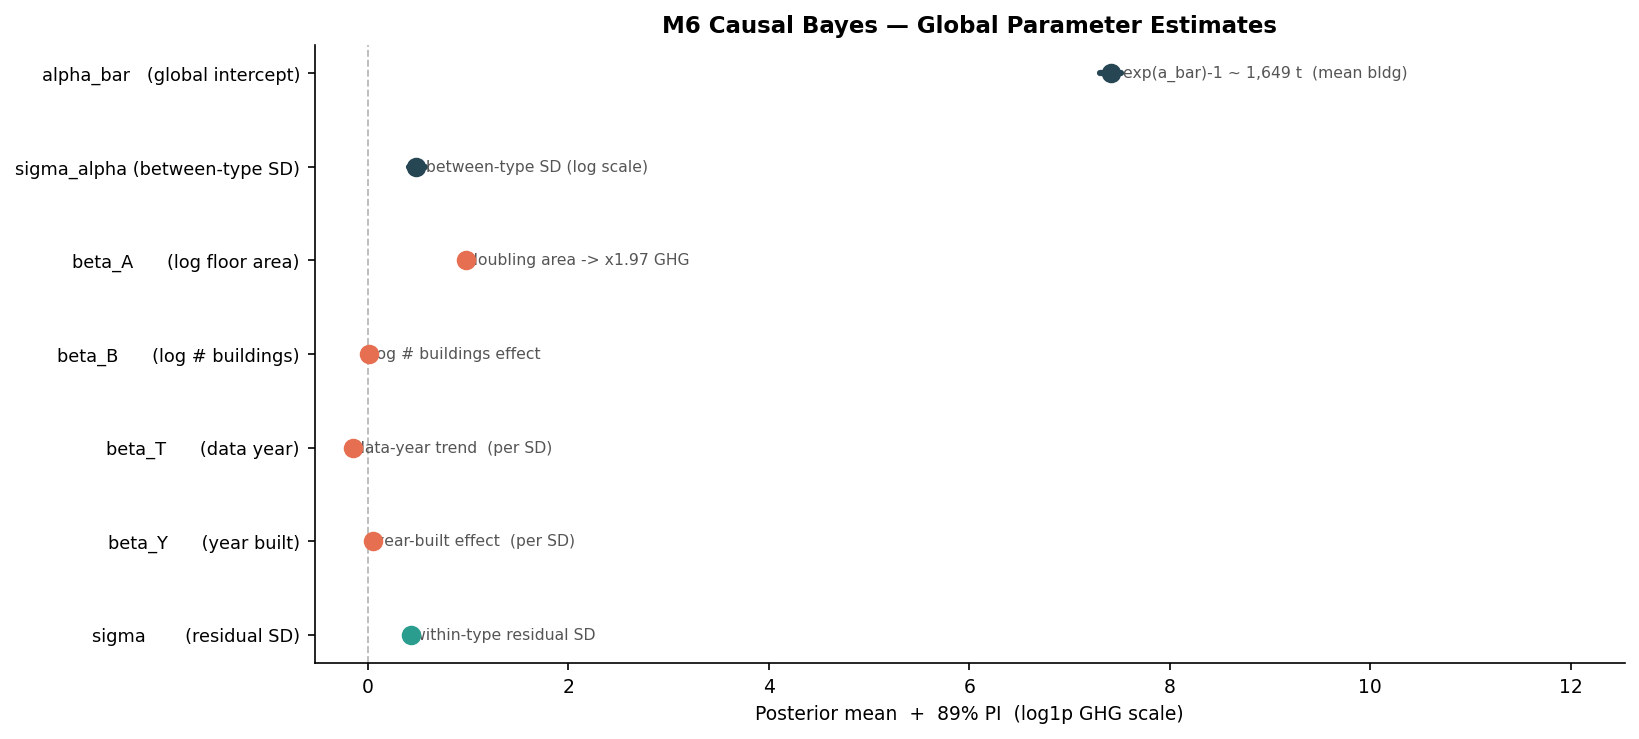
\includegraphics[width=0.95\linewidth]{figures/fig_coef_forest.png}
\caption*{\textbf{Figure 6.2. M6 global parameter estimates.} Forest plot of the seven scalar posteriors with 89\% credible intervals and back-transformed interpretations. Author's analysis of Chicago Energy Benchmarking data.}
\end{figure}

\subsection{The Property-Type Hierarchy}

Property type spans a 22-fold emissions range beyond what size, age, and reporting year explain: the 55 estimated intercepts $\alpha_j = \bar{\alpha} + \delta_j \sigma_\alpha$ run from Data Center at $+9.352$ [9.189, 9.515] down to Repair Services at $+6.234$ [6.015, 6.452], a spread of 3.1 log units. Figure 6.3 ranks all 55 types represented in the compliant training set (of the 63 the dataset records; Section 4.1).

The ordering is consistent with engineering knowledge rather than statistical accident. Data centres run power densities an order of magnitude above typical commercial space; laboratories ($+8.386$) carry ventilation and fume-hood loads around the clock; supermarkets ($+8.286$) run continuous refrigeration. At the bottom, repair services and distribution centres combine low occupancy density with intermittent conditioning. A flat model that ignored property type would be systematically wrong across this entire range, which is the empirical justification for the hierarchical structure.

The interval widths encode data availability, and that is partial pooling working as intended. Frequently reported types such as Laboratory have intervals about 0.10 log units wide; rare types carry far wider intervals: Repair Services spans 0.44 log units and Distribution Center spans 0.83. Each is accordingly shrunk toward the global mean rather than extrapolated from sparse local data. Data Center keeps a high posterior mean despite few observations because the signal is strong enough to overcome the pooling.

\begin{figure}[tbp]
\centering
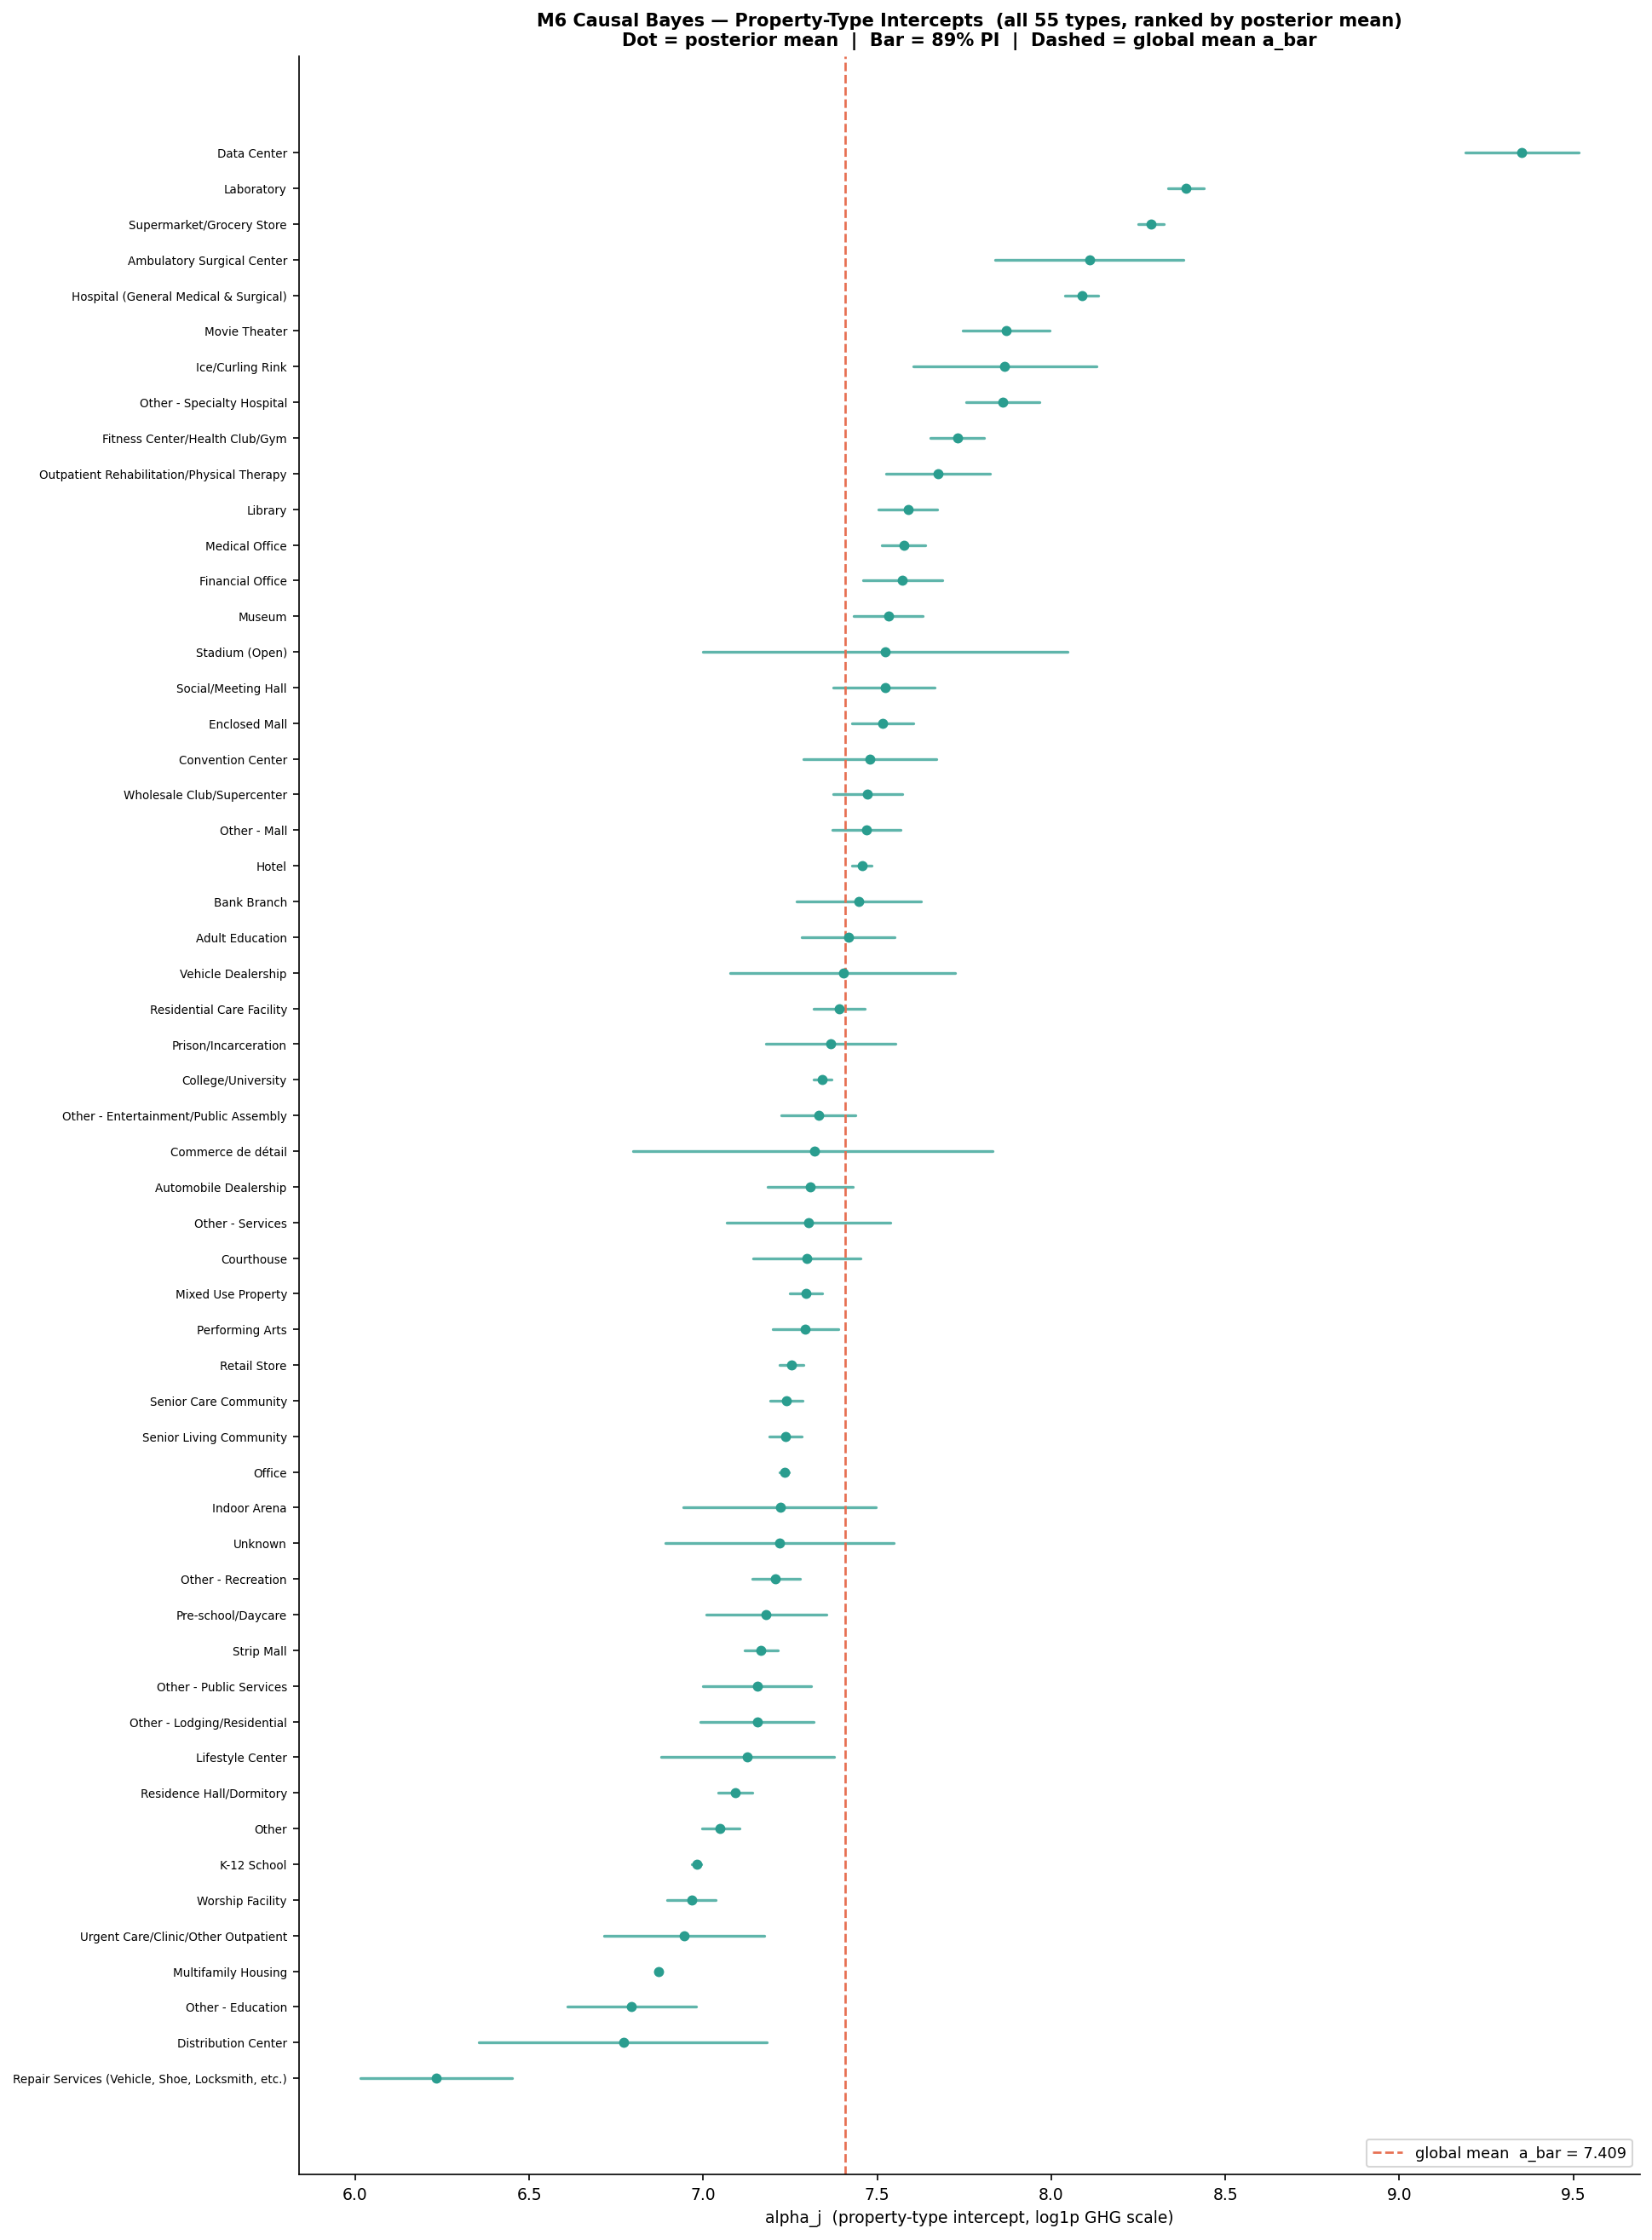
\includegraphics[width=0.8\linewidth]{figures/fig_type_intercepts.png}
\caption*{\textbf{Figure 6.3. Property-type intercepts, all 55 types.} Ranked posterior means with 89\% credible intervals for $\alpha_j$; the dashed line marks the global mean $\bar{\alpha}$. Interval width tracks how often each type appears in the compliant training set. Author's analysis of Chicago Energy Benchmarking data.}
\end{figure}

\subsection{Deployment Inference for the Non-Compliant Stock}

The deployment exercise of Section 5.6 reported point predictions; the posterior adds their uncertainty. M6 is applied to the 5,510 building-year records that never reported under the ordinance, using only their upstream features, the only inputs that exist for a non-reporting building. The posterior predictive median is 1,043 metric tons CO$_2$e against an observed compliant median of 1,018, a difference of 2.5\%, with an 89\% interval for an individual building of [495, 2,103] (Figure 6.4).

Two features of this result deserve emphasis. First, the interval is wide, roughly a factor of four, and deliberately so: without observed energy use, the residual scale $\sigma$ and the type uncertainty propagate through the posterior predictive in full, and a narrower interval would be a false promise rather than a better model. Second, non-compliant buildings predict at essentially the same emission level as compliant ones. Within the limits stated in Section 5.6 (no ground truth exists for these buildings), this is the pattern the tested DGP predicts: compliance is determined by the gate variables, not by emissions, so once the upstream features are conditioned on, non-reporting buildings should look like reporting ones. The result is consistent with selection rather than with a systematically cleaner non-reporting stock.

The per-type medians show meaningful heterogeneity beneath the aggregate: K-12 schools at 676 t and multifamily housing at 893 t sit below the global level, while mixed-use properties (2,117 t), college and university buildings (1,360 t), and offices (1,298 t) sit above it. One data feature matters for interpretation: 3,924 of the 5,510 non-compliant records (71\%) carry an Unknown property type, because a building that never filed has no recorded type. These buildings receive the global intercept with full between-type uncertainty, and their deployment median (1,021 t) accordingly sits near the global level. That is the model behaving correctly under missing type information, not a separate finding about unknown-type buildings.

\begin{figure}[tbp]
\centering
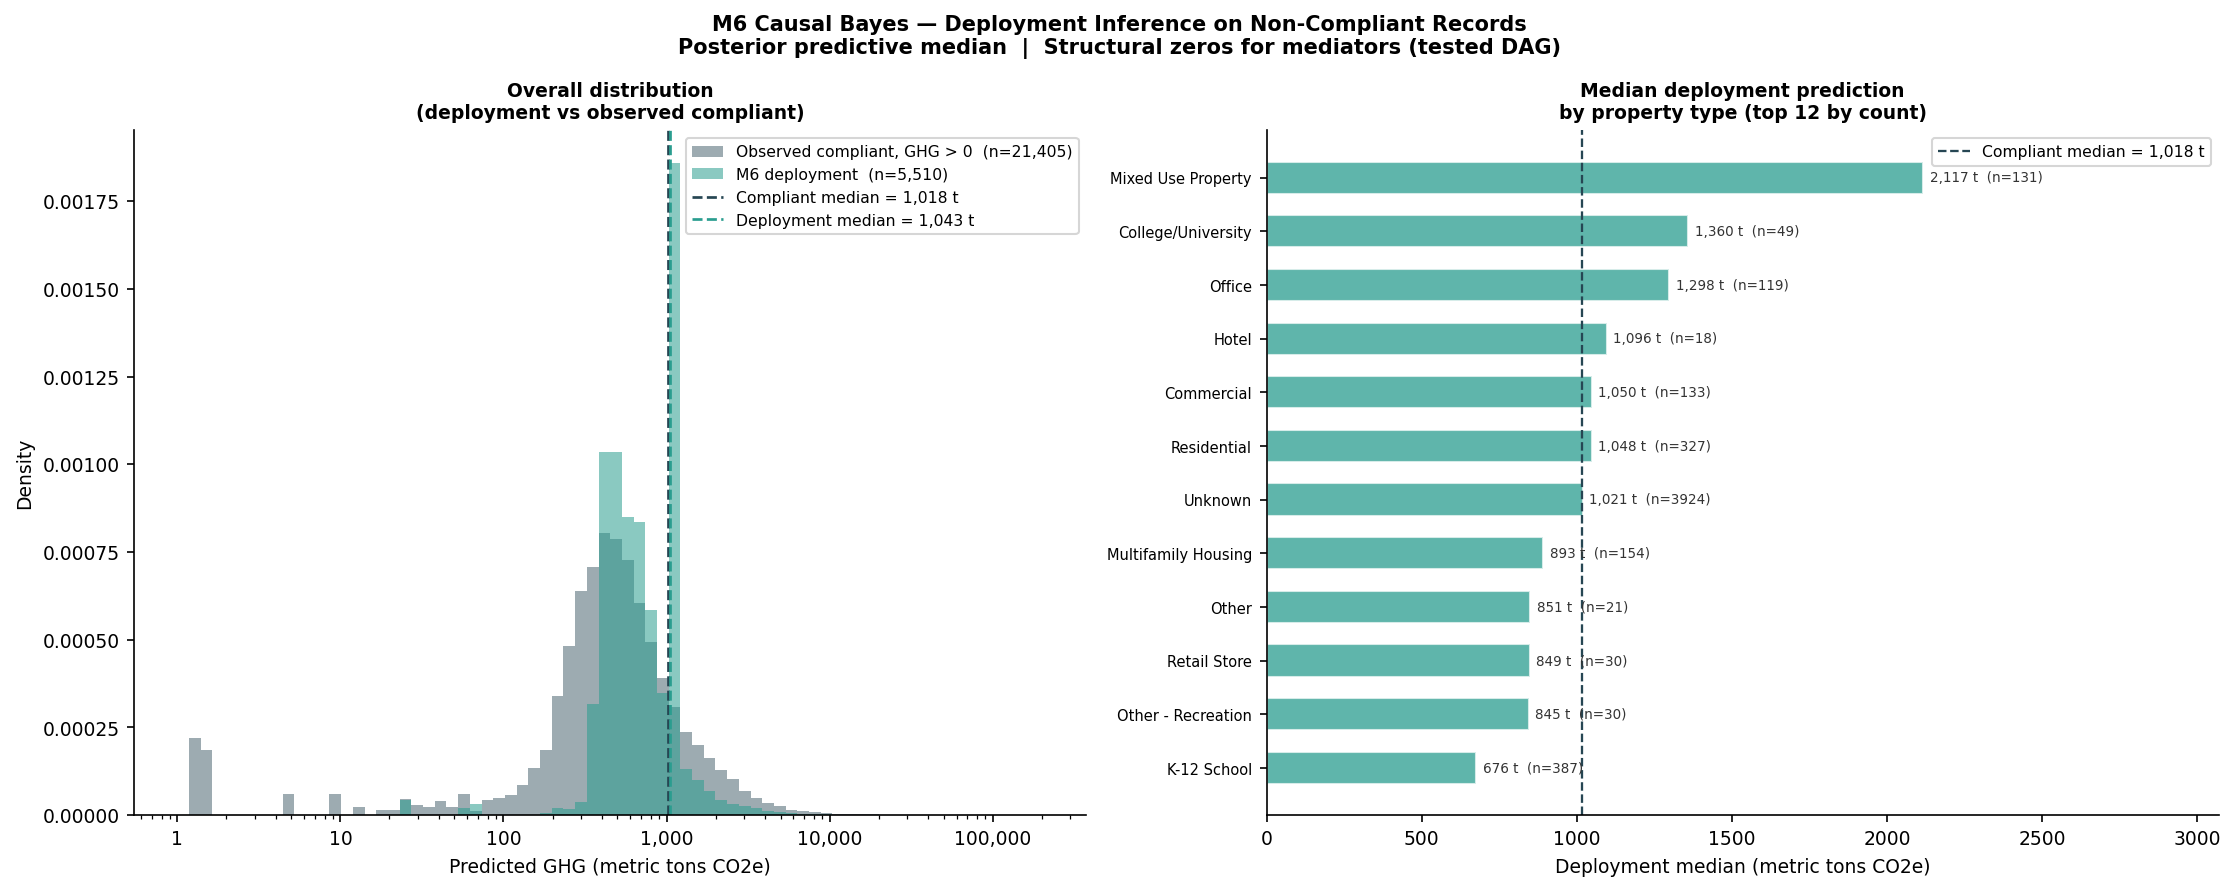
\includegraphics[width=0.95\linewidth]{figures/fig_m6_deployment.png}
\caption*{\textbf{Figure 6.4. Deployment inference for 5,510 non-compliant building-year records.} Left: posterior predictive distribution for the non-compliant stock against the observed compliant distribution, with medians marked (1,043 vs 1,018 metric tons CO$_2$e). Right: per-type deployment medians for the twelve most common non-compliant property types. Author's analysis of Chicago Energy Benchmarking data.}
\end{figure}

\subsection{Sensitivity Analysis}

The posteriors above rest on two analyst-controlled inputs: the prior specification and the IPW trim cap. The sensitivity analysis tests whether the section's findings depend on either. The design is committed ex ante, in the same spirit as the predictions of Section 5.5: the four parameters of interest ($\beta_A$, $\beta_T$, $\sigma_\alpha$, $\sigma$) and the review criterion are declared before any alternative model is fitted, so the analysis cannot select favourable specifications after the fact. The criterion flags a parameter for review when its posterior mean shifts by more than 20\% of the base 89\% credible interval half-width. The intercept prior $\bar{\alpha} \sim \text{Normal}(7.0, 1.0)$ is not varied, since it is anchored to the observed log-GHG mean of 7.08 rather than chosen freely.

Each dimension is varied independently around the base specification, which is loaded from the saved experiment trace rather than re-fitted, so the base column is identical to Table 6.1 by construction. On the prior dimension, the slope priors are tightened to $\text{Normal}(0, 0.25)$ and loosened to $\text{Normal}(0, 1.00)$ against the base $\text{Normal}(0, 0.50)$, with the scale priors varied in step. On the weighting dimension, the raw inverse propensity weights are capped at the 95th, 99th (base; \cit{colehernan2008}{Cole \& Hernán, 2008}), and 99.9th percentiles. All four alternative fits use the identical sampling specification as M6 and all converge cleanly: zero divergent transitions in every run, $\hat{R}_{\max} \leq 1.006$ across the new fits, and $\text{ESS}_{\min} \geq 460$.

The three caps produce maximum normalised weights of 1.166, 1.322, and 2.750, and the asymmetry is informative. Tightening from the 99th to the 95th percentile changes the maximum weight by only 12\%, because the weight distribution is compact in that region. Loosening to the 99.9th percentile more than doubles it, admitting a small number of buildings whose estimated compliance propensity falls below roughly 35\%, predominantly very small buildings and atypical property types, each now carrying about twice the influence of an average observation. The lenient cap is included as a deliberate stress test, not as a plausible alternative.

Table 6.2 summarises the outcome. Against prior specification, all four parameters are stable: the largest shift anywhere is 3.2\% of the interval half-width, and $\beta_A$ and $\beta_T$ are identical to three decimal places across all three prior widths. With 21,406 observations the likelihood dominates any reasonable prior; halving or doubling the prior scales produces no detectable change. The largest (still negligible) prior sensitivity belongs to $\sigma_\alpha$, as expected: the between-type standard deviation is informed by the 55 types rather than the 21,406 buildings, so its effective sample is the smallest in the model.

\par\medskip\noindent
{\small\itshape \textbf{Table 6.2. Sensitivity of the four parameters of interest.} Maximum shift in posterior mean across the alternative specifications on each dimension, expressed as a percentage of the base 89\% credible interval half-width; the review threshold is 20\%. Author's analysis of Chicago Energy Benchmarking data.\par}
\nopagebreak\medskip\nopagebreak
{
\setlength{\tabcolsep}{7pt}
\renewcommand{\arraystretch}{1.15}
\begin{longtable}{lrrr}
\toprule
Parameter & Prior shift (max) & IPW shift (max) & Assessment \\
\midrule
\endfirsthead
\toprule
Parameter & Prior shift (max) & IPW shift (max) & Assessment \\
\midrule
\endhead
\bottomrule
\endlastfoot
$\beta_A$ & 3.2\% & 29.0\% (see text) & robust \\
$\beta_T$ & 1.0\% & 11.0\% & robust \\
$\sigma_\alpha$ & 3.2\% & 1.2\% & robust \\
$\sigma$ & 0.5\% & 11.3\% & robust \\
\end{longtable}
}
\par\medskip

Against the IPW trim cap, three of the four parameters again move by at most 11.3\% of the half-width, and $\beta_T$ is the strongest result in the analysis: the data-year trend is identical to three decimal places under every cap, because a temporal signal that operates across all buildings and all years cannot be redistributed by reweighting individual observations. The one flag is $\beta_A$ under the lenient 99.9th-percentile cap, at 29\% of the half-width. The 29\% figure is inflated by the denominator, not the numerator: the absolute shift is 0.0018 (posterior mean 0.979 to 0.977), the half-width it is measured against is 0.006, and the implied change in the floor-area doubling effect is from $\times 1.971$ to $\times 1.968$, a 0.15\% difference with no analytical consequence. The mechanism is also interpretable: the extreme weights upweight small, low-propensity buildings, marginally reducing the leverage of large buildings and with it the estimated elasticity. Figure 6.5 shows the full comparison; on every panel the markers for the three specifications overlap rather than spread.

The joint conclusion is that the findings of Sections 6.2 through 6.4 are properties of the data and the tested structure, not artefacts of prior choice or weight trimming. The elasticity near one, the decarbonisation trend, the 22-fold type heterogeneity, and the residual floor all survive every specification tested, and the 99th-percentile trim of the base model, adopted from \cit{colehernan2008}{Cole and Hernán (2008)}, emerges corroborated: the aggressive and lenient caps bracket it and produce essentially the same model.

\begin{figure}[tbp]
\centering
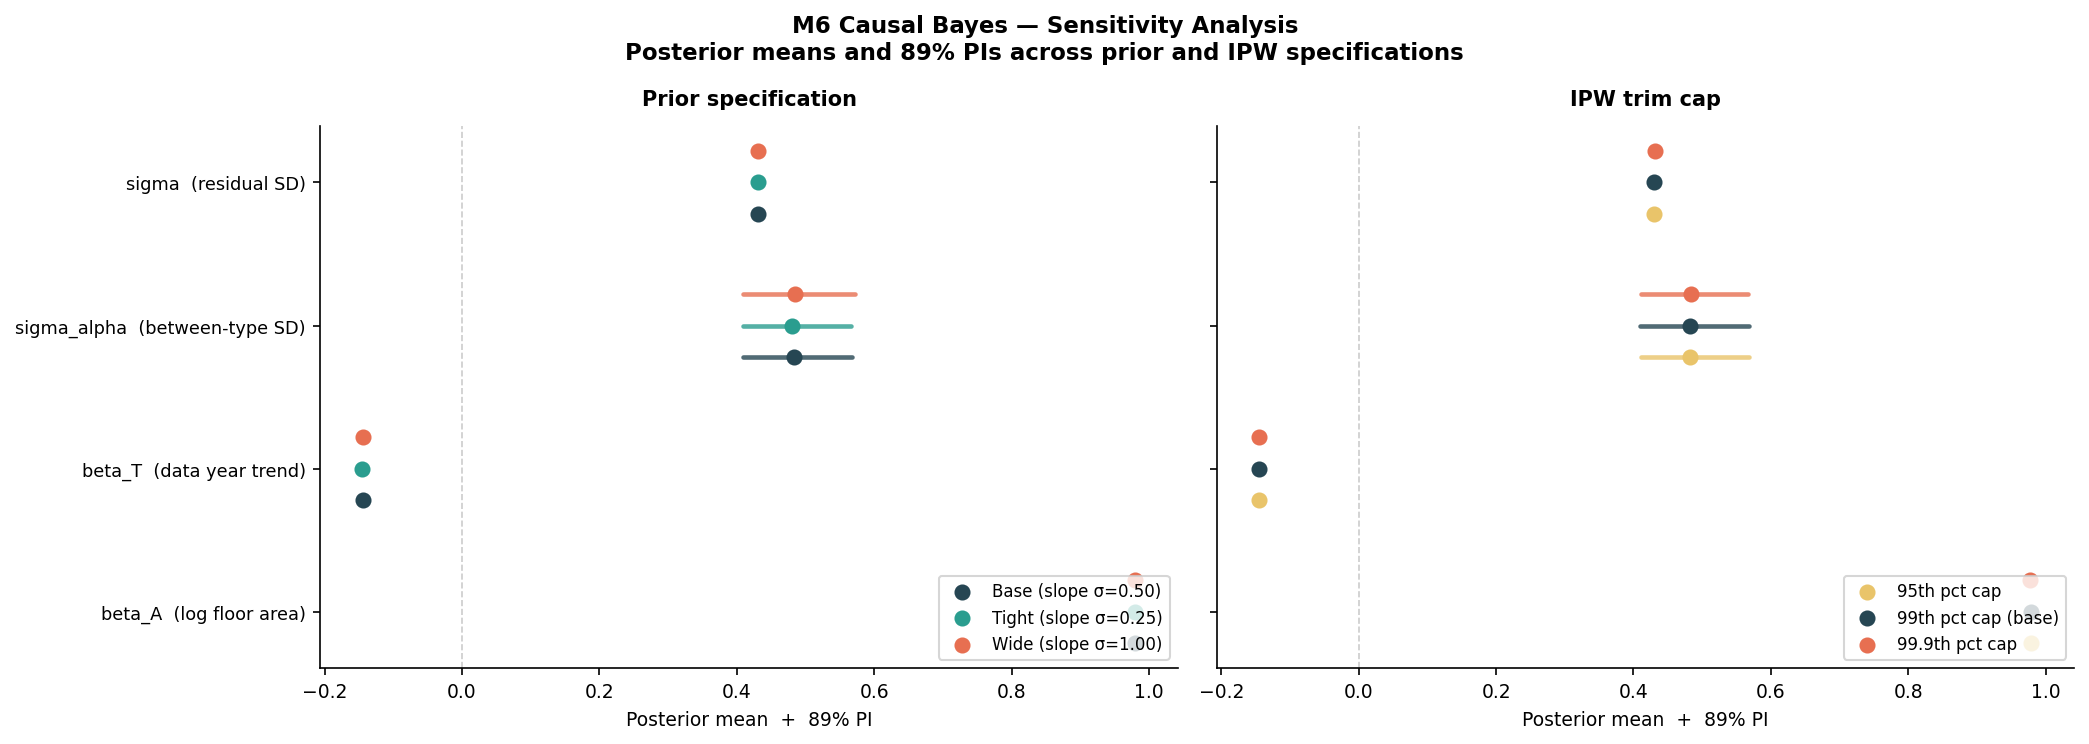
\includegraphics[width=0.95\linewidth]{figures/fig_sensitivity_forest.png}
\caption*{\textbf{Figure 6.5. Sensitivity forest plot.} Posterior means and 89\% credible intervals for $\beta_A$, $\beta_T$, $\sigma_\alpha$, and $\sigma$ across all specifications. Left: prior sensitivity (tight, base, wide; IPW fixed at the 99th percentile). Right: IPW sensitivity (95th, 99th, 99.9th percentile caps; priors fixed at base). Overlapping markers indicate robustness. Author's analysis of Chicago Energy Benchmarking data.}
\end{figure}

